\begin{savequote}[75mm]
We assume that a computer cannot deal reasonably with language unless it can understand the subject it is discussing.
\qauthor{Terry Winograd}
\end{savequote}

\chapter{Learning to Respond}

\section{Introduction}
\subsection{The Response Problem}
The true test for intelligence lies in the Response phase of the Luna Game. Players must be prepared to respond to prompts of virtually any variety. The prompts will likely be in natural language. They may be related to one another or not.  The goal of the players to produce Responses that are convincingly intelligent, thereby inducing the opponent to provide a high Guess of the player's Smarts Rating. I call this general problem \textit{The Response Problem}.

\subsubsection{Definitions and Notation}
The definitions and notation here were introduced in Chapter 4. Let $P$ be the set of all players in the LRS. Let $SR \subseteq \mathbb{R}^+$ be the domain of Smarts Ratings. I use $\Sigma^*$ to denote the set of all possible alphanumeric strings. Each player $p \in P$ is equipped with a Response Function $r_p : \Sigma^* \to \Sigma^*$ that gives the player's Response to any prompt. Each player is also equipped with a fixed finite set of prompts or questions, written $Q_p \subset \Sigma^*$. These questions are used by the player during the Interview Phase. A Guess Function, written as $g_p : \mathcal{R}_{Q} \to SR$, gives the player's Guess of an opponent's Smarts Rating based on the opponent's Responses to a set of questions $Q$.

\subsubsection{The Response Problem}
\textbf{The Response Problem:} Learn a Response Function $r : \Sigma^* \to \Sigma^*$ that maximizes $E_{p \in P}[g_p(r(Q_p))]$, the expected Guess of an opponent.

\subsubsection{Scope of the Problem}
The Response Problem is extremely difficult. Given the range of potential questions, the only way to truly solve the problem is to solve all of AI. Consider just a few possible question types:
\begin{itemize}
\item \textbf{Trivia}: What is the name of Ron Swanson's first wife in \textit{Parks and Recreation}?
\item \textbf{Commonsense}: Why not wear black while biking at night?
\item \textbf{Creativity}: Write an original poem about ducks.
\item \textbf{Opinion}: Is it really better to have loved and lost?
\item \textbf{Sensorimotor}: Turn left, left, left, and then left. Where are you now?
\item \textbf{Vision}: What does ;) look like?
\item \textbf{Emotional Intelligence}: John gives Jane a large holiday present. Jane does not give John one. How might John feel?
\item \textbf{Analysis}: A journalist writes an article subtitled ``First Sign of President's Radical Shift to the Right?'' What biases might the journalist have?
\item \textbf{Philosophy}: What does it mean to be virtuous?
\item \textbf{Open Problems}: Does P $=$ NP?
\end{itemize}

\noindent In practice, the boundaries of the Response Problem will emerge from the collective behavior of LRS players. The question types that carry the most weight will be those repeatedly asked by large factions of players. As players continue to adapt and refine their questions, any overfitted solutions, i.e. Response strategies based on only a shallow understanding of the particular questions in the system, will quickly be exposed as fraudulent. Thus the Response Problem strongly incentivizes machine player developers to focus on general AI.
 
\subsection{Related Work}
The Response Problem bears immediate resemblance to a subfield of Natural Language Processing known as Question Answering (Q\&A). Q\&A is sometimes defined as the general problem of automatically responding to any question posed in natural language (e.g. \cite{andrenucci05, hirschman01}), which suggests that Q\&A and the Response Problem are identical. However, the more common definition distinguishes Q\&A as the task of retrieving relevant information from a natural language corpus in response to a factual question (\cite{brill01, burger03, kwok01, ravichandran02, voorhees99}). The practical scope of Q\&A is much more narrow than that of the Response Problem; in contrast with the ten question type examples given in section 1.1.3, Q\&A deals almost exclusively with Trivia (see \cite{soricut04} for an exception). Most existing Q\&A systems can only hope to address a small subset of the Response Problem.

Nonetheless, researchers of the Response Problem can take inspiration and guidance from the substantial work done on Q\&A. Perhaps most enlightening is the manner in which Q\&A is decomposed into subproblems. The 2003 review by Burger et al. defines a roadmap for Q\&A that has often been followed by subsequent research \cite{burger03, kolomiyets11}. The subtasks include\footnote{There are twelve subtasks defined in \cite{burger03}, but the most notable are the first six, as the remaining six --- Real-Time Q\&A, Multilingual Q\&A, Interactive Q\&A, Advanced Q\&A, User Profiling, and Collaborative Q\&A --- go beyond the basic objective of Q\&A.} Question Classes, Question Processing, Context, Data Sources, Answer Extraction, and Answer Formulation. These six subtasks are sufficiently general that they may transfer to the Response Problem. Written two years later, the review by Andrenucci \& Sneiders distinguishes three main approaches to Q\&A: a Natural Language approach, an Information Retrieval approach, and a question template approach \cite{andrenucci05}. The three differ mainly in emphasis; the Natural Language approach focuses on the semantics of the question and answer, the Information Retrieval approach is chiefly concerned with the representation and access of information, and the question template approach deals almost exclusively with pattern matching questions and annotated information. Each of these approaches could in theory be generalized for the Response Problem, but the Natural Language approach, with its emphasis on semantics, is likely most appropriate. 

Figure \ref{fig:NLPQA}, reproduced from \cite{androutsopoulos95}, provides an example of how an end-to-end system for Q\&A can be separated into modules. The first section of the system is dedicated to linguistic processing. At the lowest level, syntax rules and a lexicon are used to parse the natural language input a standard format that a semantic interpreter can process. Semantic rules, such as first-order logic, and a world model, which encodes relationships and constraints for elements of the semantic domain, are integrated to produce a logical query into a database. After the database processes the query, a final module converts the database output into a human-readable response. This architecture offers an example of how a system for the Response Problem could be structured. The syntax rules and lexicon may be already be ready for more general use. With a sufficiently advanced collection of semantic rules, world model, and database, the system could perform quite well. Of course, the level of advancement in each of these areas required for the Response Problem seems far beyond the reach of current AI.

A system for Q\&A offers a solution to the Trivia-type questions in the Response Problem. Several other possible question types have their own corresponding areas of research. Commonsense reasoning \cite{davis15}, creativity \cite{oliveira15}, spatial reasoning \cite{freska15}, vision \cite{zheng15}, and emotional intelligence \cite{tawatsuji15} have all been formalized and are actively studied\footnote{In fact, each of the preceding citations came from 2015!} as subproblems in AI. Questions of opinion, and other questions that rely on a human identity, may be addressed with research in Dialogue, e.g. through a chatbot \cite{weizenbaum66}. One possible approach to the Response Problem is to detect the type of a question and then parcel it out to the appropriate sub solution. This method is in line with the ``bottom-up'' approach to AI. The analogous method, the development of one general mechanism for answering all questions in the Response Problem, aligns with the ``top-down'' approach. To gain insight into the current state of AI, each paradigm should be used for the Response Problem; the highest Smarts Rating of a single mechanism machine and the highest Smarts Rating of a machine that uses a combination of subproblems will both serve as illuminating indicators of progress.

\begin{figure}[h]
\centerline{%
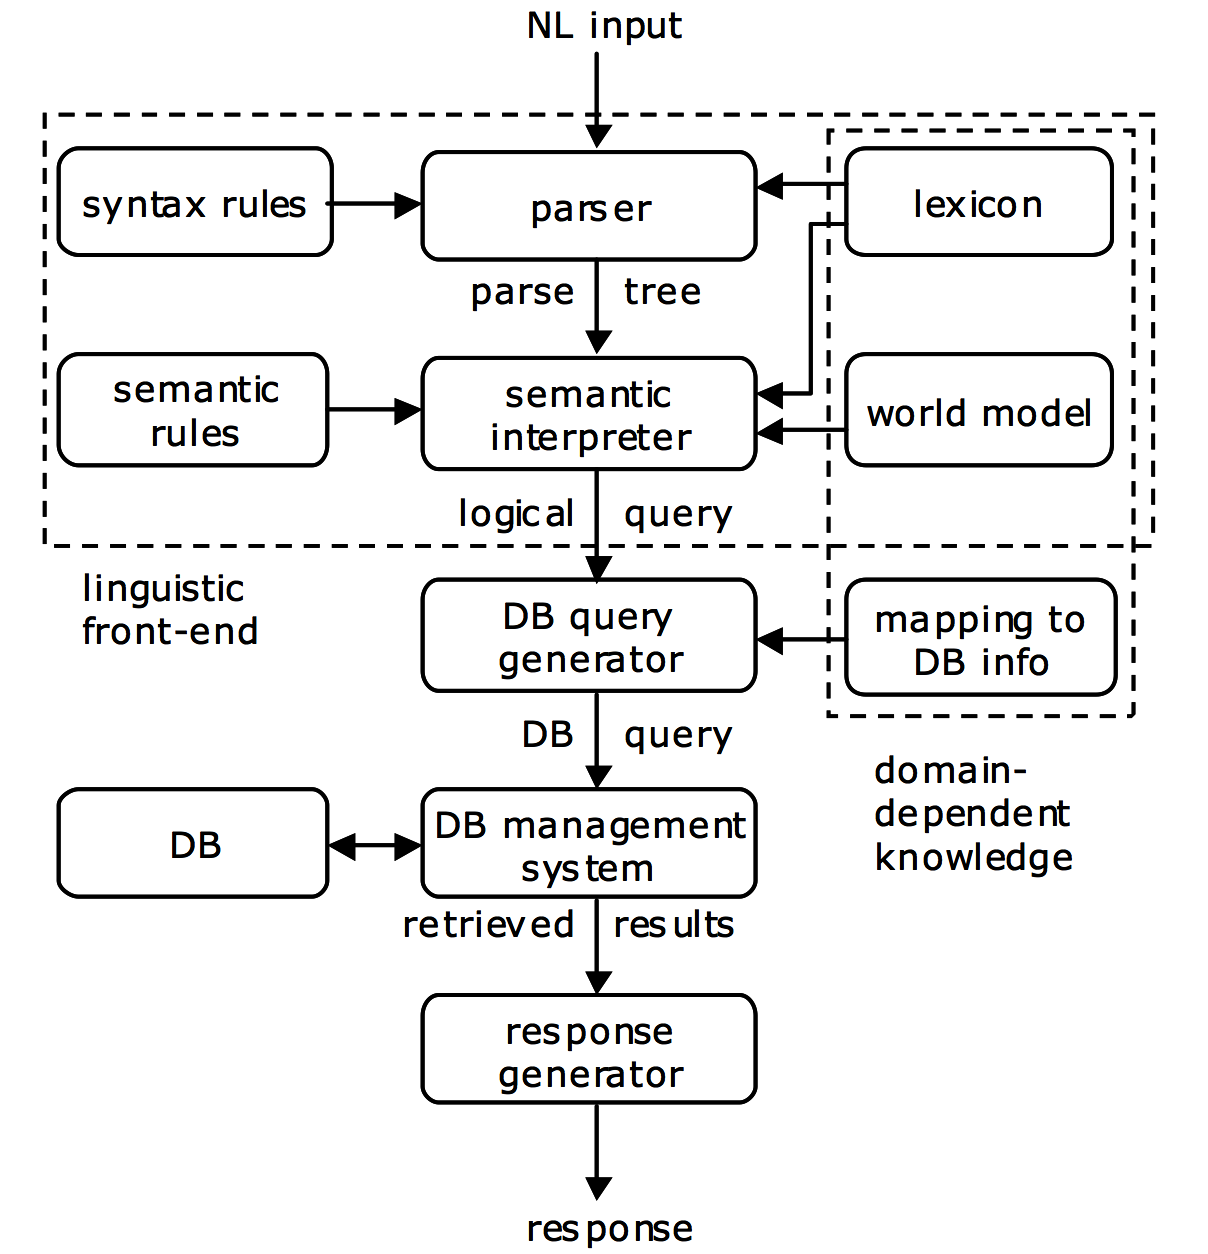
\includegraphics[width=0.5\textwidth]{figures/NLPQA.png}}%
\caption{Architecture of a typical Natural Language system for Question Answering, from \cite{androutsopoulos95}. The structure could be used in full or in part as a template for approaching the Response Problem.}
\label{fig:NLPQA}
\end{figure}

DIALOGUE

EACH TYPE OF QUESTION HAS BEEN STUDIED IN ITS OWN RIGHT

\section{Methods}
\subsection{Approaching the Response Problem}

TODO

\subsection{Example Solution}

TODO

\subsection{Datasets}

TODO

\section{Results}
TODO

\section{Discussion}TODO
%
%\pagebreak
%\bibliographystyle{abbrvnat}
%
%\begin{thebibliography}{}
%
%\bibitem{andrenucci05}
%Andrenucci, Andrea, and Eriks Sneiders. ``Automated question answering: Review of the main approaches.'' IEEE, 2005.
%
%\bibitem{androutsopoulos95}
%Androutsopoulos, Ion, Graeme D. Ritchie, and Peter Thanisch. ``Natural language interfaces to databases --- an introduction.'' Natural language engineering 1.01 (1995): 29-81.
%
%\bibitem{brill01}
%Brill, Eric, et al. ``Data-Intensive Question Answering.'' TREC. Vol. 56. 2001.
%
%\bibitem{burger03}
%Burger, John, et al. ``Issues, tasks and program structures to roadmap research in question \& answering (Q\&A).'' Document Understanding Conferences Roadmapping Documents. 2003.
%
%\bibitem{davis15}
%Davis, Ernest, and Gary Marcus. ``Commonsense reasoning and commonsense knowledge in artificial intelligence.'' Communications of the ACM 58.9 (2015): 92-103.
%
%\bibitem{freska15}
%Freksa, Christian. ``Strong spatial cognition.'' Spatial Information Theory. Springer International Publishing, 2015. 65-86.
%
%\bibitem{hirschman01}
%Hirschman, Lynette, and Robert Gaizauskas. ``Natural language question answering: the view from here.'' natural language engineering 7.04 (2001): 275-300.
%
%\bibitem{kolomiyets11}
%Kolomiyets, Oleksandr, and Marie-Francine Moens. ``A survey on question answering technology from an information retrieval perspective.'' Information Sciences 181.24 (2011): 5412-5434.
%
%\bibitem{kwok01}
%Kwok, Cody, Oren Etzioni, and Daniel S. Weld. ``Scaling question answering to the web.'' ACM Transactions on Information Systems (TOIS) 19.3 (2001): 242-262.
%
%\bibitem{oliveira15}
%Oliveira, Hugo Gon�alo, and Am�lcar Cardoso. ``Poetry Generation with PoeTryMe.'' Computational Creativity Research: Towards Creative Machines. Atlantis Press, 2015. 243-266.
%
%\bibitem{ravichandran02}
%Ravichandran, Deepak, and Eduard Hovy. ``Learning surface text patterns for a question answering system.'' Proceedings of the 40th Annual Meeting on Association for Computational Linguistics. Association for Computational Linguistics, 2002.
%
%\bibitem{soricut04}
%Soricut, Radu, and Eric Brill. ``Automatic Question Answering: Beyond the Factoid.'' HLT-NAACL. 2004.
%
%\bibitem{tawatsuji15}
%Tawatsuji, Yoshimasa, Keiichi Muramatsu, and Tatsunori Matsui. ``Qualitative description representing brain functional connection for human emotional states toward human-like agents.'' Transactions of the Japanese Society for Artificial Intelligence 30.5 (2015): 626-638.
%
%\bibitem{voorhees99}
%Voorhees, Ellen M. ``The TREC-8 Question Answering Track Report.'' TREC. Vol. 99. 1999.
%
%\bibitem{weizenbaum66}
%Weizenbaum, Joseph. ``ELIZA --- a computer program for the study of natural language communication between man and machine.'' Communications of the ACM 9.1 (1966): 36-45.
%
%\bibitem{zheng15}
%Zheng, Yufeng, Erik Blasch, and Adel S. Elmaghraby. ``Biologically Inspired Methods for Imaging, Cognition, Vision, and Intelligence.'' Computational Intelligence and Neuroscience 501 (2015): 154816.
%
%\end{thebibliography}
%
%\end{document}